% !TeX root = main.tex
% !TeX spellcheck = it_IT
\frontmatter
\setcounter{page}{1}
\pagenumbering{Roman}
\tableofcontents
\chapter{Introduzione}
aha ciaoo
\mainmatter
\setcounter{page}{1}
\pagenumbering{arabic}
\pagestyle{fancy}
\makeatletter
\let\ps@plain\ps@fancy
\makeatother
\chapter{Cenni biografici}
\section{Montreal: l'infanzia e gli inizi}
Paul Bley nacque a Montreal, in Quebec, il 10 Novembre 1932. I genitori adottivi furono Betty Marcovitch, emigrata rumena di modeste origini, e il facoltoso imprenditore tessile Joe Bley\footcite[10]{stopping}. Paul era in verità figlio biologico di Joe e di una sua dipendente (una donna del Canada francese di nome Lucie): dal momento che Betty non poteva avere figli, Bley fece mettere il neonato in orfanotrofio per convincere poi la moglie, ignara della situazione, ad adottarlo; la madre biologica di Paul venne poi assunta come balia dalla famiglia. Lo stesso Paul non sarebbe venuto a conoscenza di questo fatto fino a molti anni dopo, nel 1992\footcite[13]{stopping}. La madre adottiva, in ogni caso, crebbe il bambino con affetto e cura, decidendo di impartirgli un'educazione musicale e di fargli frequentare la scuola della comunità ebraica di Montreal.\par
La rivelazione del fatto di essere stato adottato (nonostante entrambi i genitori biologici fossero in realtà presenti nel suo nucleo familiare) fu un evento traumatico per il bambino, tanto più che allo stress causato dalla situazione si aggiunse quello provocato dal divorzio dei genitori nel 1939. Il giovane Paul, per far fronte alla mancanza di un senso di appartenenza, trovò così rifugio nella musica e non a caso il pianista ricorda come in quegli anni (anche grazie al suo insegnante August Dècarie) maturò in lui la decisione di diventare un musicista professionista\footcite[15]{stopping}. Sempre in quel periodo Paul ebbe il suo primo contatto con il concetto di improvvisazione:
\begin{fquote}
	Oltre alla scuola, stavo iniziando a studiare per il mio Bar Mitzvah per il quale avrei dovuto cantare un testo in ebraico. Quando chiesi al mio rabbino ``Come fa la melodia?'' egli rispose ``Inventala sul momento\footnote{\cite[16]{stopping}. Le traduzioni dall'inglese di questo (e altri) documenti in questo elaborato sono proprie.}''.
\end{fquote}
Giovanissimo, Bley trova impiego come pianista di varietà al locale della Young Men's Hebrew Association dove venne in contatto con le strutture e le sonorità della musica popolare. Viene in seguito assoldato da altri locali in cui spesso è chiamato a suonare anche con musicisti molto più anziani di lui.
A quattordici anni forma il suo primo gruppo, i \textit{Buzzy Bley}: l'esperienza gli permette di iniziare a farsi conoscere a Montreal e di sviluppare la capacità di gestire, economicamente ed artisticamente, un gruppo di musicisti. \\
Il contatto con il jazz avvenne con la \textit{tramp band} di Al Cowan\footnote{Al Cowan (asse da bucato), B.T. Lundy (sax tenore), Buddy Jordan (tromba), Walter Bacon (batteria). Le \textit{tramp band} erano complessi da intrattenimento che suonavano spesso strumenti bizzari quali, per l'appunto, l'asse da bucato.}, alle cui esibizioni Bley spesso assisteva dopo aver finito di suonare nei locali in cui era ingaggiato. Il gruppo spesso invitava il giovane pianista a suonare e Bley ricorda le dinamiche di apprendimento che venivano a formarsi in quei contesti, tra nottate in locali frequentati da giocatori d'azzardo e prostitute.\par
Nel 1948 Bley potè assistere a un concerto del pianista suo concittadino Oscar Peterson, che nonostante avesse all'epoca solo ventitrè anni già mostrava i segni di un talento geniale e fuori dalla norma, come già all'epoca riconosciuto da Bley\footcite[20]{stopping}. Peterson, a sua volta, rimase impressionato da Bley tanto da chiedergli, alle porte della sua partenza per gli Stati Uniti nel 1949, di sostituirlo come pianista per finire il suo contratto all'Alberta Lounge con il suo bassista e il suo batterista\footnote{Rispettivamente Ozzie Roberts e Clarence Jones.}. Questa fu solo una delle prime fortuite occasioni che, peculiarmente, sarebbero state una costante della vita di Bley. Egli, a suo merito, seppe sempre sfruttarle in maniera congrua.\\
Suonando allo Chalet Hotel Bley venne in contatto con la cantante newyorkese Nina Grey, che lo spinse e lo supportò insieme alla madre Betty nel seguire il proprio sogno di trasferirsi a New York per frequentare la Juilliard School per la musica e le arti a Manhattan. \par
\section{New York e la Juilliard: le prime esperienze}
Nel 1950 Bley si trasferì dunque a New York, dove poté immergersi nella florida scena jazzistica dell'epoca ascoltando le esibizioni di nomi di primissimo rilievo come Charlie Parker, Max Roach, Miles Davis ma anche Lennie Tristano, Lee Konitz e Billy Bauer.\\
Alla Juilliard Bley riceve un'educazione di impostazione moderna, soprattutto in ambito compositivo\footcite[23]{stopping}. Questi anni formativi lasciarono un'impronta profonda sulla sua concezione di tempo, tonalità e soprattutto sul rifiuto della dicotomia, tipica del jazz di quegli anni, di compositore-esecutore.
\begin{fquote}
	Il grande mistero non era se sarebbe arrivata la musica atonale, ma bensì \textit{perchè non fosse ancora arrivata}. [...] A questo riguardo la musica classica ci aveva portati fuori strada, poiché ci aveva spinti a credere che questa svolta sarebbe stata compiuta dai compositori. Nel jazz [...] un compositore è semplicemente qualcuno che non sa suonare in tempo reale.\footcite[24]{stopping}
\end{fquote}
L'atonalità e l'avanguardia, anche attraverso gli insegnamenti del compositore canadese Henry Brant\footcite[23]{stopping} esercitò da subito il proprio fascino su Bley così come su altri musicisti della scuola (come Gil Evans, George Russell e Johnny Carisi che il pianista ebbe modo di conoscere). Alla Juilliard Bley si unì alla \textit{New Jazz Society}, che si riuniva al Downbeat Club dove erano soliti suonare Parker e Charles Mingus. Quest'ultimo, in particolare, fece la conoscenza di Bley proprio in queste occasioni.\\
Durante questo periodo, chiaramente, Bley non si fece mancare numerosi ingaggi sopratutto a Brooklyn e a Long Island\footcite[47]{cappelletti} dove cementò la sua familiarità con figure quali il già citato Parker, Jackie McLean e Donald Byrd; grazie al suo manager Monte Kay suonò inoltre per diversi mesi con Lester Young\footcite[47]{cappelletti}.\par
Nonostante la fruttuosa permanenza a New York, Bley non abbandonò completamente Montreal, dividendo la propria vita tra le due città negli anni tra il 1950 e il 1953. Nella città canadese Bley si organizzò insieme ad altri due pianisti suoi concittadini, Keith White e Art Roberts, per dare forma al Jazz Workshop. Lo scopo dell'associazione era quello di creare un ambiente di sperimentazione e sviluppo e allo stesso tempo quello di iniettare nuova vita nella scena di Montreal chiamando illustri ospiti da oltre il confine. Si trattò di un'altra azione ``imprenditoriale'' da parte di Bley che durante la sua vita dimostrò sempre una certa inclinazione verso gli aspetti più gestionali della vita del musicista. Tra gli ospiti statunitensi ospitati dal Workshop ci furono Chuck Wayne, Sonny Rollins, Jackie McLean, Art Taylor e, nel 1953, perfino Charlie Parker. Il successo riscosso dell'associazione attirò l'attenzione della televisione canadese CBC che ne trasmise in diretta diversi concerti, compreso quello in cui prese parte Parker\footnote{Queste registrazioni sono disponibili nel disco \textbf{Charlie Parker - \textit{Montreal 1953}} [Uptown Records 1993]. Questo album, nelle tracce 9, 10, 11 e 12 contiene la prima registrazione del pianoforte di Bley, con Neil Michaud (basso), Ted Paskert (batteria), Dick Garcia (chitarra) e Brew Moore (sax tenore).}. Bley ricorda la differenza tra la scena di Montreal, in cui i musicisti esperti si facevano paternalmente carico dell'istruzione di quelli più giovani, e quella di New York. ``\textit{I giovani musicisti non si consideravano discepoli e la conoscenza dei musicisti più anziani era disponibile solo in vendita. Se volevo che Charlie Parker suonasse con me dovevo ingaggiarlo}\footcite[31]{stopping}''. A riprova della sua inclinazione manageriale, Bley si fece carico di scortare un Parker stralunato e ormai in preda alla propria tossicodipendenza da New York a Montreal (temendo che si sarebbe perso in aeroporto e sarebbe finito in Alaska). Parker deve aver apprezzato il pianismo di Bley, poichè lo richiamò in seguito per un ingaggio a Brooklyn\footcite[34]{stopping}. L'esperienza con Parker segnò profondamente Bley, che rimase profondamente colpito da come il sassofonista riuscisse a ``\textit{prevedere ciò che stava arrivando e pensare sempre in anticipo}''\footcite[35]{stopping}.\par
Nel 1953 Charles Mingues chiamò Bley per una registrazione come direttore d'orchestra\footnote{Composta da Janet Thurlow (voce), Charles Mingus (basso), Kenny Clarke (batteria), John Lewis (pianoforte), Ernie Royal (tromba), Danny Bank (sax baritono), Willy Dennis (trombone), Eddie Caine (sax contralto e flauto), Teo Macero (sax tenore) e Jackson Wiley (violoncello).} per alcuni pezzi nel contesto di un progetto della neonata etichetta discografica di proprietà di Mingus, la Debut Records. A questo ingaggio Mingus aggiunse un'ulteriore registrazione in trio con Art Blakey. Quest'ultima prova, pubblicata come \textbf{Paul Bley - \textit{Introducing Paul Bley}} [Debut 1954] nonostante la \textit{line-up} di primo livello appare piuttosto sbiadita e priva di carica, tanto che Cappelletti insinua che fosse stata proposta da Mingus più come forma di ringraziamento per il lavoro di direzione di orchestra che come dichiarazione di fiducia nelle doti pianistiche di Bley\footcite[49]{cappelletti}.\par
\section{L'esperienza free: Coleman, Russell, Giuffre, Rollins}
Nel 1955 Bley ricevette un ingaggio da Chet Baker per un tour di esibizioni ad Hollywood; nel 1956 venne chiamato dalla cantante Dakota Staton per poi iniziare un tour del Midwest americano con Lennie McBrown (batteria) e Hal Gaylor (basso a cinque corde)\footcite[49]{stopping}. Nello stesso anno al Birdland di New York fece la conoscenza di Karen Borg (destinata a diventare nota come Carla Bley e a essere, per un periodo, moglie di Paul), che all'epoca lavorava nel locale come cameriera. \\
In generale quello in California fu un periodo molto intenso per Bley, tanto che nel 1957 ebbe un malore e fu ricoverato per un'emorragia interna causata da un'ulcera duodenale. Bley attribuisce\footcite[54]{stopping} l'episodio al suo continuo stato di irrequietezza, nato con la rivelazione di essere stato adottato, che lo spingeva a trascurare la propria salute fisica e mentale a vantaggio degli impegni lavorativi. In seguito all'episodio Bley sostiene di aver realizzato la maggiore importanza dello stato artistico della musica jazz rispetto alla propria carriera individuale. Dopo il ricovero Bley viene raggiunto a Los Angeles da Karen Borg, con la quale aveva iniziato una relazione da qualche tempo, per poi sposarsi e stabilirsi in California.\par
Nel 1957 ottenne un ingaggio all'Hillcrest Club sul Washington Boulevard a Los Angeles con Gaylor e McBrowne a cui si aggiunse Dave Pike (vibrafono). Parallelamente approfondisce inoltre la strada dell'improvvisazione libera in duo con il trombettista Herbie Spanier\footcite[58]{stopping}. Dovendo sostituire Gaylor, che aveva deciso di trasferirsi a est, McBrowne presentò a Bley il contrabbassista Charlie Haden. Ricorda Bley: ``\textit{Charlie arrivò scalzo. Non solo non aveva le scarpe, ma anche la sua scelta di note lasciava abbastanza a desiderare. Il suo modo di tenere il tempo era impeccabile [...] sarebbe stato facile trovare un altro bassista che suonava le note corrette ma avrei dovuto essere molto fortunato per trovare un altro bassista con un senso del tempo così}\footcite[62]{stopping}''. Poco dopo anche McBrowne tornò ad est sotto ingaggio di Horace Silver e fu così sostituito da Billy Higgins che completò così la sezione ritmica. Una sera quest'ultimo propose a Bley di conoscere un trombettista e un sassofonista con cui lui e Haden stavano lavorando: si trattava, ovviamente, di Don Cherry e di Ornette Coleman.
\begin{fquote}
	Il fatto che fosse successo in una notte qualunque di un ingaggio di due anni fu una sorpresa, ma non servì più di un secondo per capire che quello era l'anello mancante tra suonare in maniera totalmente \textit{free}, senza vincoli di sorta, e suonare \textit{bebop} con cambi di accordi e tempo stabile.\footcite[64]{stopping}
\end{fquote}
Bley iniziò così la sua esperienza con Coleman (che gli sarebbe costata il posto di lavoro all'Hillcrest\footcite[51]{cappelletti}) esplorando diverse concezioni di tempo, struttura (Bley aveva sempre mal sopportato la ridondanza di sezioni A e B nella forma canzone tradizionale) e armonia. Parte di queste performance, che Bley registrava su nastro, sono documentate dai dischi \textbf{\textit{The Fabulous Paul Bley Quintet}} [America Records 1970] e \textbf{\textit{Ornette Classics 1}} [Improvising Artists 1977]. \par
Dopo un breve ingaggio con Scott LaFaro (basso), Bobby Hutcherson (vibrafono) e Larance Marable (batteria), Carla e Paul tornarono a New York nel 1959 dove la fama di Coleman precedeva il nome di Bley\footcite[70]{stopping}. Nel 1960 venne chiamato da George Russell, che aveva avuto modo di ascoltare Bley qualche tempo addietro alla Lenox School of Jazz, per un progetto di un pezzo per due pianoforti e Orchestra per la Decca Records in quello che sarebbe poi uscito con il titolo di \textit{\textbf{Jazz in the Space Age}} [Decca 1960]. Compositore affermato, Russell aveva concepito una teoria armonica basata sulla \textit{gravità tonale}\footcite[3]{russell} e su un'organizzazione tonale incentrata sul cromatismo interpretato come naturale estensione della serie armonica\footcite[12]{russell}, prospettiva che senza dubbio ben si complementava con la fuga dalla tonalità (benchè Russell di fatto proponesse un \textit{rafforzamento} parossistico del concetto di tonalità) che caratterizzava la musica di Coleman.\\
L'altro pianista chiamato a realizzare il progetto era Bill Evans, in quegli anni all'apice della sua popolarità dopo le registrazioni di \textit{\textbf{A Kind Of Blue}} [Columbia 1959]. Bley racconta stupito di come questi si era inaspettatamente rivelato in sintonia con le sue idee di sperimentazione e atonalità, tanto da preoccuparsi che Evans potesse rubargli la scena e lasciarlo senza lavoro. Con suo grande sollievo, però, Bley racconta che dopo le registrazioni andò ad ascoltare il trio di Evans al Village Vanguard per scoprire che il pianista, al di là dell'esperienza con Russell, non sembrava interessato ad allontanarsi da quella che era la sua zona di comfort\footcite[75]{stopping}.\par
In questi anni Bley conobbe il bassista Steve Swallow, con il quale si ritrovò a suonare in diverse occasioni in duo. Contestualmente, fu anche chiamato dal chitarrista Jim Hall per sostituirlo in un trio con il clarinettista e sassofonista Jimmy Giuffre e il bassista Ralph Peña. Giuffre, così come Russell, aveva avuto modo di ascoltare Bley alla Lenox School of Jazz ed era intrigato dallo stile anticonvenzionale del pianista. In seguito all'abbandono di Peña, Bley convinse Giuffre ad assumere Swallow come bassista. Soddisfatto dal suono del trio, Giuffre portò il gruppo per una (sfortunata\footcite[77]{stopping}) tournee in Europa nel 1961. Dello stesso anno sono i due dischi che documentano questa iterazione dei \textit{Jimmy Giuffre 3}, cioè \textit{\textbf{Thesis}} [Verve 1961] e \textit{\textbf{Fusion}} [Verve 1961], in cui già si nota una prevalenza di brani scritti da Carla Bley (tendenza, questa, che non avrebbe mai abbandonato Paul nemmeno dopo la separazione).\\
In seguito a una proposta di Herbie Hancock nel 1963 Bley fu ingaggiato da Sonny Rollins insieme a Henry Grimes (basso) e Roy McCurdy (batteria) per una serie di concerti, un tour in Giappone e Stati Uniti e un disco per la RCA con Coleman Hawkins, \textit{\textbf{Sonny meets Hawk!}} [RCA Victor 1963]. A differenza delle esperienze precedenti, il repertorio di Rollins era costituito principalmente da \textit{standard} seppur suonati con grande libertà armonica e strutturale. Questa occasione diede a Bley l'opportunità di misurarsi con un ulteriore approccio al linguaggio \textit{free}: il legame tra gli \textit{standard} e il pianista sarebbe continuato anche in seguito, fino alla fine della sua carriera.
\section{La maturità artistica: il trio, l'incontro con l'elettronica e il solo}
Nel 1964 Bley fu assoldato dal bassista Gary Peacock per una doppia serata: il primo concerto insieme a John Gilmore (sax tenore) e a Paul Motian (batteria) e il secondo con Albert Ayler (sax tenore) e Sunny Murray (batteria)\footcite[89]{stopping}. L'esperienza con Murray, primo batterista \textit{free} con cui Bley avesse mai avuto a che fare, fu allo stesso tempo rivelatrice e traumatica, tanto che Bley dovette chiedere a Carla di riscrivere i propri brani affinché si adattassero meglio allo stile del batterista. Non a caso, Bley avrebbe poi nella propria carriera prediletto lo stile più controllato di Motian. Gli sforzi di questa fase della carriera di Bley sono documentati nei dischi \textit{\textbf{Turning point}} [Improvising Artists 1975] con il primo quartetto e \textit{\textbf{Barrage}} [ESP-disk 1964] con Marshall Allen (sax contralto), Dewey Johnson (tromba), Eddie Gomez (basso) e Milford Graves (batteria).\par
Nello stesso anno Bley fu invitato dal trombettista Bill Dixon a prendere parte agli incontri dell'associazione Jazz Composer Guild. L'idea dell'associazione era quella di formare una sorta di sindacato per opporsi alle pratiche scorrette dei \textit{leader} delle formazioni e delle etichette discografiche. Seppur riluttante all'inizio\footnote{``L'incontro era un manipolo di anime in pena. Alla faccia della terapia di gruppo...'' \cite{stopping}, p. 91.}, Bley si ritrovò insieme al trombonista Roswell Rudd alla direzione dell'associazione in seguito alla defezione di Dixon. Durante questa nuova esperienza da organizzatore e gestore Bley riuscì a produrre diversi concerti e a guadagnare nuovi membri (tra tutti, il pianista Cecil Taylor). Il nuovo successo dell'organizzazione permetteva anche a musicisti meno noti, come a quel tempo il quintetto di Carla Bley con il trombettista (e futuro marito di Carla) Mike Mantler, di godere di un'utile visibilità. In quegli anni Carla Bley, sotto consiglio di Paul, potè utilizzare i leader delle formazioni nella Jazz Composer's Guild per formare la Jazz Composer's Orchestra Association insieme a Mantler. Bley ricorda ``Un'idea così buona da costarmi una moglie''\footcite[95]{stopping}, dato che nel 1965 Paul e Carla divorziarono.\par
In seguito alla sofferta separazione, iniziò per Bley un approfondimento della forma e delle potenzialità della formazione in trio\footcite[98]{stopping}. Il primo passo in questa direzione, \textit{\textbf{Closer}} [ESP-disk 1965] con il già citato Steve Swallow e Barry Altcschul (batteria). Per il disco Bley adottò, in controtendenza con il \textit{free} dell'epoca, la scelta di limitare la lunghezza dei soli ottenendo così una \textit{tracklist} più folta e con una maggiore varietà di temi e atmosfere\footnote{Bley, tra i cui difetti non si può certo annoverare la modestia, equipara \textit{Closer} ai dischi di Albert Ayler a livello di importanza storica per il jazz. \cite[100]{stopping}.}. Grazie al sostegno della ESP, Bley potè portare il proprio trio (con Kent Carter al basso) in Europa per un tour nello stesso anno).\par
Nel 1966 Bley iniziò una relazione (poi in seguito matrimonio) con la compositrice e pioniera della musica elettronica Annette Peacock (ex moglie del bassista Gary Peacock). Come con Carla Bley, Peacock sarebbe divenuta una presenza molto importante nella vita personale e artistica di Bley, che avrebbe suonato sue composizioni (al pari di quelle della prima moglie) per il resto della propria carriera. Nello stesso periodo Bley e Peacock si recarono in Europa insieme ad altri nomi della scena (tra cui Steve Lacy, Altschul e Carla Bley).\\
Paradossalmente, in Europa Bley trovò sempre un'accoglienza migliore rispetto agli stati uniti. Dopo un festival a Madrid con Altschul e Mark Levinson (basso), Bley fu invitato a Bologna da cui poi nacque un tour di sei mesi per l'Italia\footcite[102]{stopping}. Come altre personalità quali Steve Lacy e Don Cherry, Bley e Peacock risiedettero per qualche a tempo a Roma sotto l'egida del produttore RCA Alberto Alberti\footcite[104]{stopping}. Dall'esperienza nacque il disco in trio \textit{\textbf{Ramblin'}} [RCA Italia 1966]. Dopo altre esperienze sui palchi europei nello stesso anno (con cinque dischi dal vivo e in studio rilasciati durante il periodo), Bley ricorda come nella formazione in trio aveva finalmente trovato un campo espressivo in cui sentirsi libero:
\begin{fquote}
	Suonavo tutto io. Niente fiati. Finalmente potevo mettere in pratica le \text{mie} idee di free jazz. [...] Questo trio poteva aprire le finestre e dare ossigeno a tradizioni che avevano raggiunto un blocco.\footcite[106]{stopping}
\end{fquote}
Nel 1969 l'attenzione di Bley venne catturata dai sintetizzatori con tastiera (che iniziavano in quegli anni ad apparire sul mercato). Dopo aver convinto Robert Moog in persona a procurargli uno dei pochi esemplari di sintetizzatore semi-modulare in produzione dall'azienda\footcite[110]{stopping}, Bley e Peacock iniziarono ad esplorare le potenzialità dello strumento. I due iniziarono una serie di esibizioni (il \textit{Bley - Peacock synthesizer show} in cui Peacock, tra l'altro, fu pioniera della tecnica della sintesi vocale) anche in Europa. In particolare, Peacock fu notata da David Bowie proprio in virtù delle sue sperimentazioni vocali. I risultati di queste esplorazioni sono negli album \textbf{\textit{Improvisie}} [America 1971], \textit{\textbf{Dual Unity}} [Freedom Records 1972] e il primo album solista di Peacock \textit{\textbf{I am the one}} [RCA 1972]. La fine di questo periodo marcò anche la fine della relazione tra Bley e Peacock.\par
Nello stesso anno il discografico Manfred Eicher, della casa tedesca ECM, propose a Bley un disco in pianoforte solo per il catalogo dedicato\footcite[119]{stopping} (in cui già facevano novero Chick Corea e Keith Jarrett). Nonostante Bley non avesse mai prodotto nessun lavoro nella forma del piano solo, il risultante \textit{\textbf{Open, to Love}} è considerato uno dei punti più significativi della carriera del pianista\footcite[75]{cappelletti}. Il disco, contente brani di Carla Bley, di Peacock e dello stesso Paul, offre una summa della proposta pianistica dell'artista condensata in una forma ancora più diretta del trio.\par
Durante una permanenza a Copenhagen dove Bley registrò con il bassista autoctono Niels-Henning Ørsted Pedersen il disco \textit{\textbf{Paul Bley/NHØP}} [SteepleChase Records 1973], il pianista conobbe l'artista visuale Carol Goss, che sarebbe diventata la sua terza (e ultima) moglie. Dopo essere scampato a un incendio nella sua abitazione di New York (durante il quale Bley rischiò la vita per salvare il sintetizzatore in cui a suo dire non era nemmeno più interessato\footcite[120]{stopping}), Bley e Gross fondarono la compagnia di registrazioni audio-video Improvising Artists Inc. la cui idea era quella di invitare piccole ensemble di musicisti di estrazione trasversale al \textit{free} come Sun Ra, Sam Rivers o Lee Konitz. Curiosamente, la prima registrazione esistente degli allora giovanissimi Jaco Pastorius e Pat Metheny appartiene proprio alla neonata etichetta di Bley (il disco \textit{\textbf{Jaco}} [Improvising Artists 1974]). L'etichetta fu anche promotrice dei primi pioneristici esperimenti di perfomance audio-visiva in ambito jazz ad opera di Goss: n particolare nel 1977 Sun Ra e Bley presero parte a questa performance ibrida di musisciti e sintetizzatori video\footcite[129]{stopping}. In quel periodo, il successo dei dischi più orientati a un sound elettrico (non solo della sua etichetta, ma in generale per le direzioni intraprese da pianisti come Joe Zawinul, Herbie Hancock e Chick Corea) spinse Bley a scegliere di differenziarsi focalizzando i suoi sforzi sul pianoforte acustico\footcite[127]{stopping}. \par
Dopo sette anni di attività discografica, Bley e Goss decisero di chiudere la società per concentrarsi sulla propria produzione artistica e sul proprio matrimonio\footcite[132]{stopping}.\par
\section{Il tramonto della carriera: tour e insegnamento}
L'esperienza di \textit{business} maturata negli anni e il fitto network di conoscenze tra musicisti di Bley gli permisero, alla soglia degli anni '80, di intraprendere una fitta stagione di concerti e di \textit{reunion.} Tra queste, una sfortunata tournée con Chet Baker nel 1985 (trent'anni dopo la loro prima collaborazione), in cui Bley ebbe l'esperienza di un trombettista ormai non più in condizione di reggere un tour a causa della sua tossicodipendenza\footcite[137]{stopping}. \\
Nel 1989 l'editor del \textit{Jazz Magazine} parigino Phillipe Carles organizzò una riunione del progetto Jimmy Giuffre 3 con Steve Swallow (ora al basso elettrico e marito di Carla Bley) in Europa, dove a differenza degli anni '60 venne ora accolto tra gli onori generali\footcite[137]{stopping}. Dall'esperienza furono prodotti i dischi \textit{\textbf{The Life of a Trio: Saturday}} [Owl Records 1990] e \textit{\textbf{The Life of a Trio: Sunday}} [Owl Records 1990]. \par
È a questo periodo che risale la fase più prolifica, a livello di registrazioni, di Bley: adducendo come causa di questo nuovo desiderio di entrare in sala di registrazione il fatto di aver ridotto al minimo le occasioni di suonare. Questi anni di attività corrispondono anche a un approccio più rilassato e meno competitivo di Bley rispetto alla pratica pianistica e alla scena jazz\footcite[82]{cappelletti}.\par
Nel 1993 Bley ritorna eccezionalmente al sintetizzatore (questa volta, però, digitale) ventidue anni dopo il suo ultimo disco elettronico nel 1971\footcite[148]{stopping}
. Il risultato è \textit{\textbf{Synth-Thesis}} [Postcard Records 1993]. Nello stesso anno, nonostante le proprie reticenze verso l'insegnamento, accetta una sporadica cattedra al Conservatorio del New England a Boston (lo stesso dove Giuffre aveva insegnato per anni). Tra i suoi allievi più illustri figurano la pianista giapponese Satoko Fujii e il compositore israeliano Yitzhak Yedid.\par
Paul Bley morì il 3 gennaio 2016 nella sua casa a Stuart, in Florida, di cause naturali.
\chapter{L'estetica pianistica e improvvisativa}
\section{Sulle orme di Ornette}
\begin{fquote}
	Non sono mai stato un amante degli accordi. Ho sempre pensato che un accordo fosse una melodia verticale suonata simultaneamente: se un accordo non poteva essere dissezionato in maniera tale che ogni nota si allineasse a formare una melodia di senso compiuto, non era un buon accordo.\footcite[71]{stopping}
\end{fquote}
Una delle caratteristiche più lampanti dello stile improvvisativo di Bley risiede senza dubbio nel suo approccio, che fonde in uno stile ``polifonico''\footcite[50]{cappelletti} concezioni di natura melodica e armonica. \par
È interessante notare come anche nella prima fase della carriera di Bley, più legata al linguaggio bebop e all'armonia tradizionale, vi fossero già delle caratteristiche tipiche anche dei lavori successivi\footcite[104]{dean}. Ad esempio, nel primo disco di Bley da solista \textit{Introducing Paul Bley} [Debut 1953] con Art Blakey e Charles Mingus, si nota già una spiccata tendenza alla manipolazione armonica. Ad esempio, l'introduzione di \textit{I Can't Get Started} (in figura \ref{fig:cant}) mostra già quello che probabilmente è l'influsso degli insegnamenti di Brant, con una chiara impronta polifonica dell'andamento delle due mani e una scelta di intervalli dal suono scuro e dissonante.
Si tratta ancora, chiaramente, di una sperimentazione piuttosto marginale (e in ogni caso meno avanzata dei risultati che ad esempio Lennie Tristano aveva ottenuto in anni precedenti). \\
Emerge già in ogni caso, come punto di rottura con il linguaggio melodico bebop da cui Bley ancora attinge (e attingerà in seguito) a piene mani, la tendenza a cercare ed ostentare un senso di continuità con lunghe frasi melodiche monoritmiche, spesso anche monofoniche, che si estendono spesso anche oltre la struttura di pertinenza. È interessante, a tal proposito, notare come già in questo album si riscontra la tendenza di Bley all'esporre i temi in maniera minima, senza armonizzazioni o \textit{block chords} di sorta.
\begin{figure}[H]
	\centering
	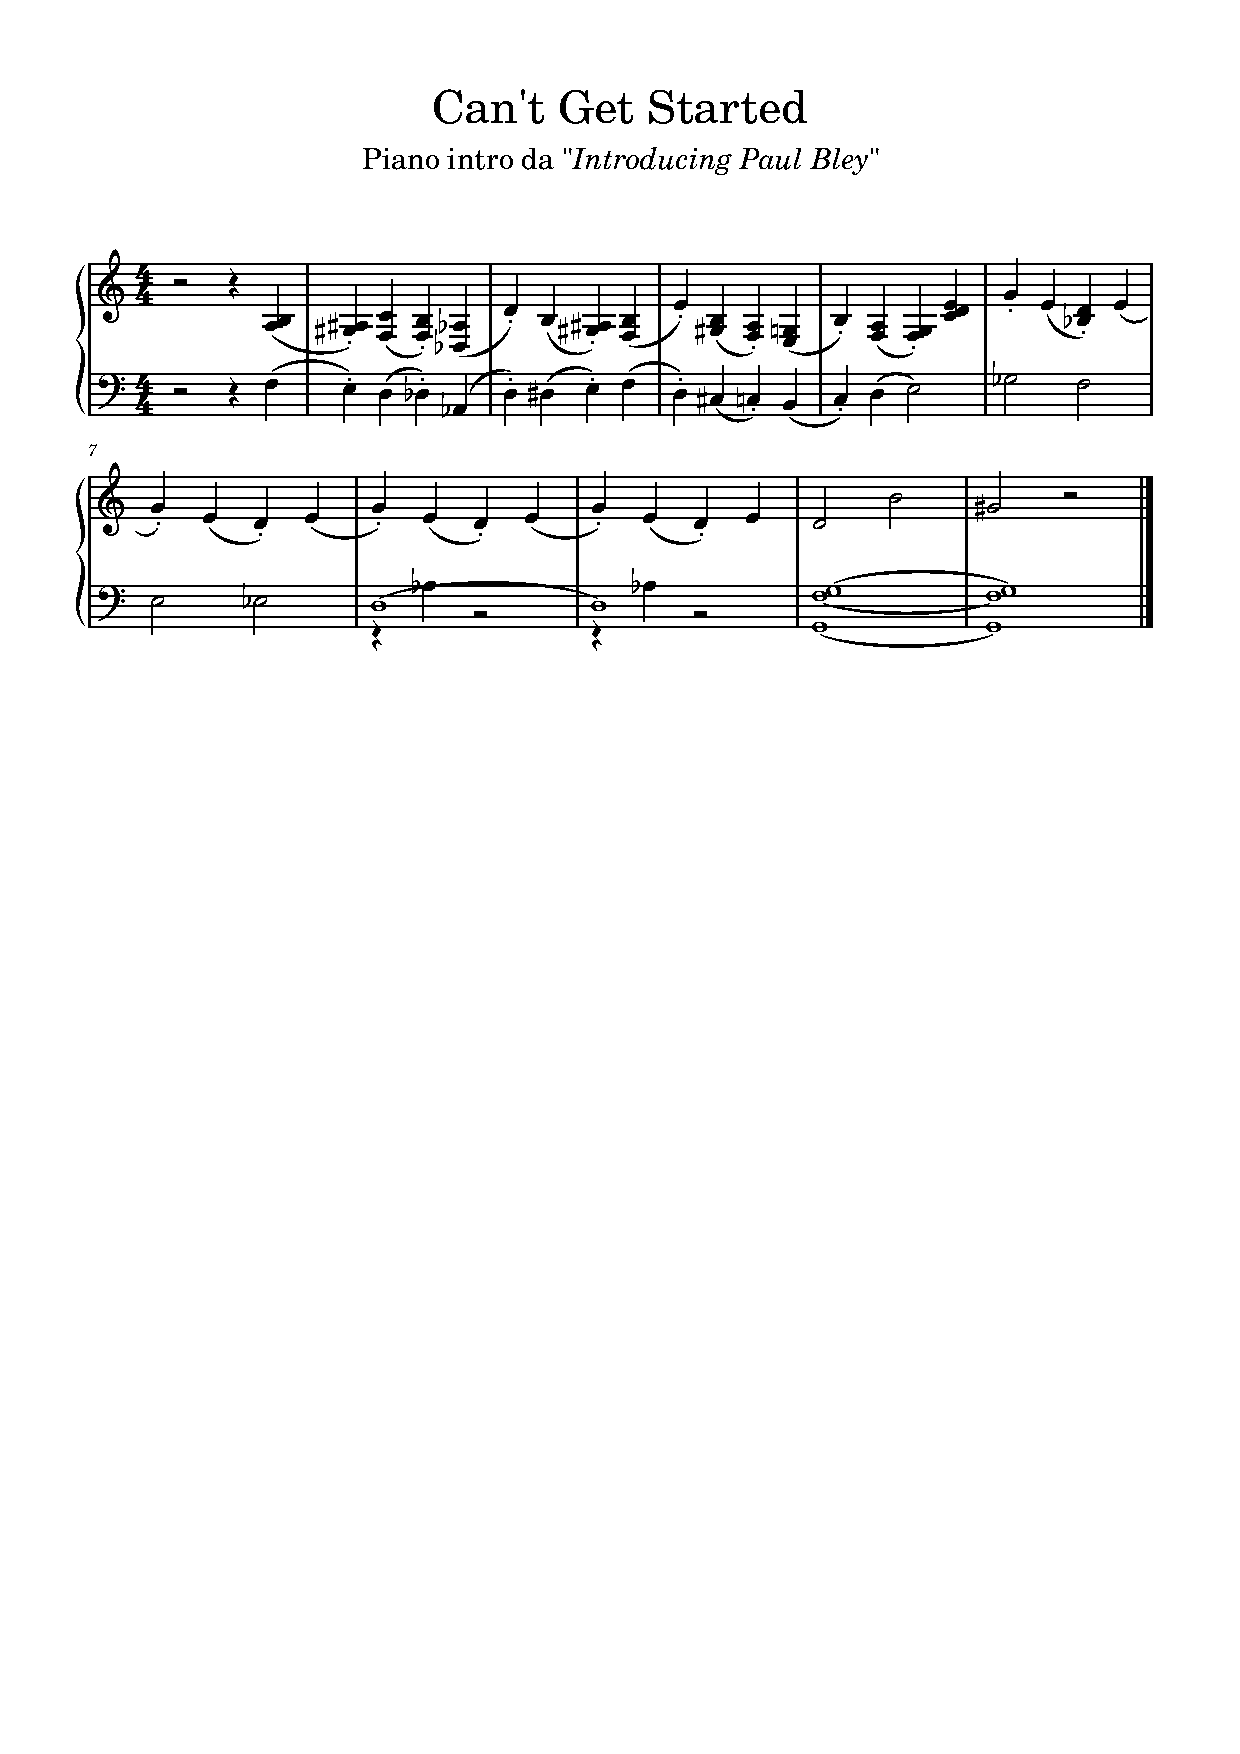
\includegraphics[clip,trim=1cm 18cm 1cm 4.3cm, width=.85\textwidth]{cantgetintro.pdf}
	\caption{Introduzione di \textit{I can't Get Started} da \textit{Introducing Paul Bley}}
	\label{fig:cant}
\end{figure}
Chiaramente, l'incontro con Coleman può essere visto come la scintilla che porta davvero Bley ad abbracciare il linguaggio free; è bene ricordare, però, che il linguaggio entro cui Bley si muove è sempre prettamente jazz e il cordone ombelicale della continuità con la tradizione non viene mai davvero reciso. L'impiego delle forme bebop come l'abbassamento della quinta o della terza sugli accordi di dominante o i circondamenti delle note accordali è ricorrente e sistemico sia prima che dopo il contatto con Coleman\footcite[26]{meehan}. Bley fa spesso uso delle scale esatonali (come si può sentire in tutte le registrazioni con Jimmy Giuffre nel 1961), delle scale alterate e soprattutto del linguaggio blues.\\
\begin{figure}[h]
	\centering
	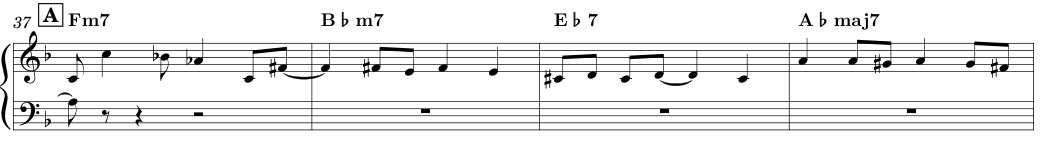
\includegraphics[width=0.9\linewidth]{screenshot001}
	\caption{Esempio di utilizzo di scala esatonale nel solo di \textit{All the things you are} nel disco \textit{Sonny Meets Hawk!}}
	\label{fig:screenshot001}
\end{figure}   
In particolare, vale la pena di approfondire l'evidente ascendente che la musica di Coleman ha evidentemente esercitato per tutta la vita del pianista.
\begin{fquote}
	Ornette ha risolto, con una singola mossa, un problema che era in fase di accumulazione da dieci anni. Ciò consisteva nel capire cosa fare per rendere l'improvvisazione jazz più interessante. Bird era un virtuoso sui cambi armonici e dopo di lui ne sono arrivati a dozzine. Non c'era niente di rimasto da suonare: ciò che avevi era una forma canzone di trentadue battute, una più una meno, che era ormai consunta come base su cui suonare. Quindi, ciò che Ornette fece fu dire che dopo la melodia tu dovevi suonare su solo uno dei centri tonali della melodia. Scriveva i temi deliberatamente in modo tale che non ci fossero trentadue battute di cambi armonici equamente distribuiti. Suonavano come se fossero tonali, ma a un esame più approfondito della composizione le battute erano irregolari e cose così.\footcite[12]{downbeat74}
\end{fquote}
Anche per Coleman, così come per Bley, si può notare il suo vocabolario musicale sia in fin dei conti direttamente mutuato da quello swing, bebop e rhythm \& blues e che l'operazione effettivamente innovativa consista nel nuovo significato dato dalla combinazione di questi motivi tradizionali in nuovi pattern metrici e melodici: l'innovazione non sta quindi nella creazione di un nuovo vocabolario ma bensì nella ridefinizione della sintassi e della grammatica musicale\footcite[109]{cogswell}. Senza alcun dubbio questa tendenza era compatibile con la determinazione di Bley di rimanere, in ogni caso, nell'ambito di un campo comunicativo jazzistico. La già citata continuità nelle frasi di Bley costituisce un altro punto in comune con l'estetica di Coleman, in cui emerge una volontà quasi metodica di mettere in relazione ogni motivo con quello precedente e quello successivo\footcite[115]{cogswell}. In questo senso la continuità melodica di Bley in tutte le fasi della carriera lo ha sempre contraddistinto se messo a confronto con pianisti quali Cecil Taylor, per cui invece vi è il tentativo di scardinare la coerenza non solo del linguaggio pianistico, ma anche della tecnica. In questo senso lo stile solistico di Bley è fortemente melodico non tanto rispetto all'armonia intesa in senso boppistico (che Bley, molto spesso, sceglie di non seguire) quanto più in relazione alla continuità interna del fraseggio. In Bley vi è spesso un fluire ininterrotto di idee melodiche che vengono concatenate, elise e combinate\footcite[20]{meehan}. Armonicamente, le continue escursioni di tonalità di Bley, che però non si incanala mai in una vera e propria bitonalità o politonalità, potrebbero rientrare nel concetto di \textit{pantonalità}\footcite[73]{reti} che in contrasto con l'atonalità propriamente definita, in cui il concetto stesso di tensione e rilascio armonico è effettivamente reso nullo, mostra una continua produzione e rilascio di dissonanze senza una reale soluzione di continuità.\par
Un altro concetto Colemaniano che ha probabilmente esercitato una forte influenza sul pianista è quello di \textit{erasure phrases}, che Bley spiega come ``frasi che erano tonali e ben temperate [alternate a] frasi che invece non lo erano deliberatamente\footcite[67]{stopping}'' con lo scopo di ``cancellare dalla tua memoria ciò che hai appena ascoltato.[...] Non sono lì per dirti qualcosa ma per farti dimenticare. Sono lì per farti sciacquare la bocca\footcite[32]{meehan}''. Ovviamente, per il pianoforte, strumento temperato per eccellenza, era impossibile riprodurre le variazioni microtonali di intonazione che caratterizzavano lo stile di Coleman; a tal proposito Bley sviluppa una metodologia personale per dare l'effetto di \textit{erasure phrase} in diversi punti dei propri soli. Come si può notare nelle trascrizioni dei soli di \textit{Ramblin'} (fig. \ref{fig:ramblin}) e \textit{All The Things You Are}, Bley spesso si trova a suonare passaggi che sono composti da frammenti di materiale tonale ad alta densità di note che, di conseguenza, eludono un centro tonale esatto e offuscano il senso armonico imitando la sensazione di disorientamento data dalle frasi non temperate suonate da Coleman. L'ambiguità riguarda anche l'aspetto ritmico: queste frasi sono spesso costituite da una scarica fitta di note senza una scansione ritmica regolare, con frequenti micro-interruzioni, inciampi, accelerazioni e ritenuti. Sono definibili come \textit{gesti}, piuttosto che vere e proprie melodie con coerenza interna, posti tra due idee melodiche dotate invece di autosufficienza e rilevanza.\par 
A tal proposito appare inevitabile, per Bley, la riflessione sui limiti intrinseci allo strumento del pianoforte quando messo a confronto con la libertà timbrica e di intonazione del sassofono.
\begin{fquote}
	Spendevo tre quarti del tempo facendo accordare Ornette per vedere se sarei riuscito a fargli suonare il la a 440 Hz... Purtroppo io non avevo la stessa flessibilità che aveva lui quando si trattava di suonare un la.\footcite[62]{litweiler}
\end{fquote}
L'interrogazione sui limiti timbrici del pianoforte, unita alla teoria, anch'essa mutuata da Coleman, della mancanza di equivalenza dei toni a diverse ottave (per la quale una stessa nota a ottave differenti non dovrebbe essere considerata, appunto, la ``stessa'' nota\footcite[110]{dean}) avrebbe portato Bley a esplorare i suoni interni del pianoforte (tecnica usata, ad esempio, in \textit{Olhos de Gato} in \textit{\textbf{Alone, again}} [Improvising Artists 1976] in cui la cordiera del pianoforte viene pizzicata o in \textit{Touching 1} da \textit{\textbf{Mr. Joy}} [Mercury 1968] dove Bley opera una sorta di glissato sulle corde individuali). Sempre questa ricerca di nuove possibilità al di là del rigido temperamento del pianoforte sarebbe stata, con tutta probabilità, anche la chiave dell'interessamento agli strumenti elettronici negli anni '70.\par
Bley aveva inoltre sempre mal sopportato la ripetitività della forma canzone\footnote{``{Se ci metti un minuto a suonare una sezione AABA hai già suonato tre sezioni ridondanti nel primo minuto. Tenere questo passo per quindici minuti, con tre sezioni A al minuto, è ridondanza all'estremo}.'' \cite[25]{stopping}} e aveva cercato nella dissoluzione della struttura una risposta a questa esigenza interpretativa, con il risultato che questo approccio rischiava di portare a un vicolo cieco dal momento che ``[suonare] \textit{totalmente free} non ti permetteva necessariamente di continuare [...], fine del concerto''; l'esperienza all'Hillcrest con Coleman fu in questo senso illuminante: 
\begin{fquote}
	suggeriva [una struttura del tipo] ABCDEFGHIJK in cui la ripetizione era un anatema. Non era completamente free perchè completamente free significava una sezione A per sempre in metamorfosi. Era una forma che aveva senso perchè tu finalmente potevi tornare alla musica scritta e il pubblico aveva qualcosa a cui aggrapparsi.\footcite{hamilton}
\end{fquote}
In questo modo si può dire che Coleman avesse offerto un modo di comporre spontaneamente attraverso l'improvvisazione melodie in emergenza da quella originale, generando nuovi pattern basato sulla direzione, velocità o sul materiale melodico dell'originale\footcite[305]{gluck}. La connessione biunivoca tra composizione e improvvisazione è sempre stata cara a Bley\footcite[22]{cappelletti} e non è un caso, in fin dei conti, che egli sia stato uno dei pochi pianisti con cui Coleman abbia mai suonato (oltre a Joachim Kuhn e Geri Allen). Forse il già citato approccio orizzontale all'armonia ben si sposava con la libertà richiesta da Ornette nell'accompagnamento.\par
In particolare, questo sincretismo tra tradizione, innovazione, linguaggio blues e concezione Colemaniana si presenta all'ascoltatore analizzando gli ultimi due \textit{chorus} di solo di piano di \textit{Ramblin'} dall'omonimo album registrato in Italia nel 1966 (in figura \ref{fig:ramblin}). In questo blues dalla forma aperta (che però Bley in questo disco approccia con una maggiore fedeltà alla struttura classica a dodici battute) appare evidente come si passi con relativa disinvoltura da un vocabolario strettamente blues a invece un fraseggio lungo, spezzato e non rispettoso della struttura armonica. \par 
\begin{figure}[h]
	\centering
	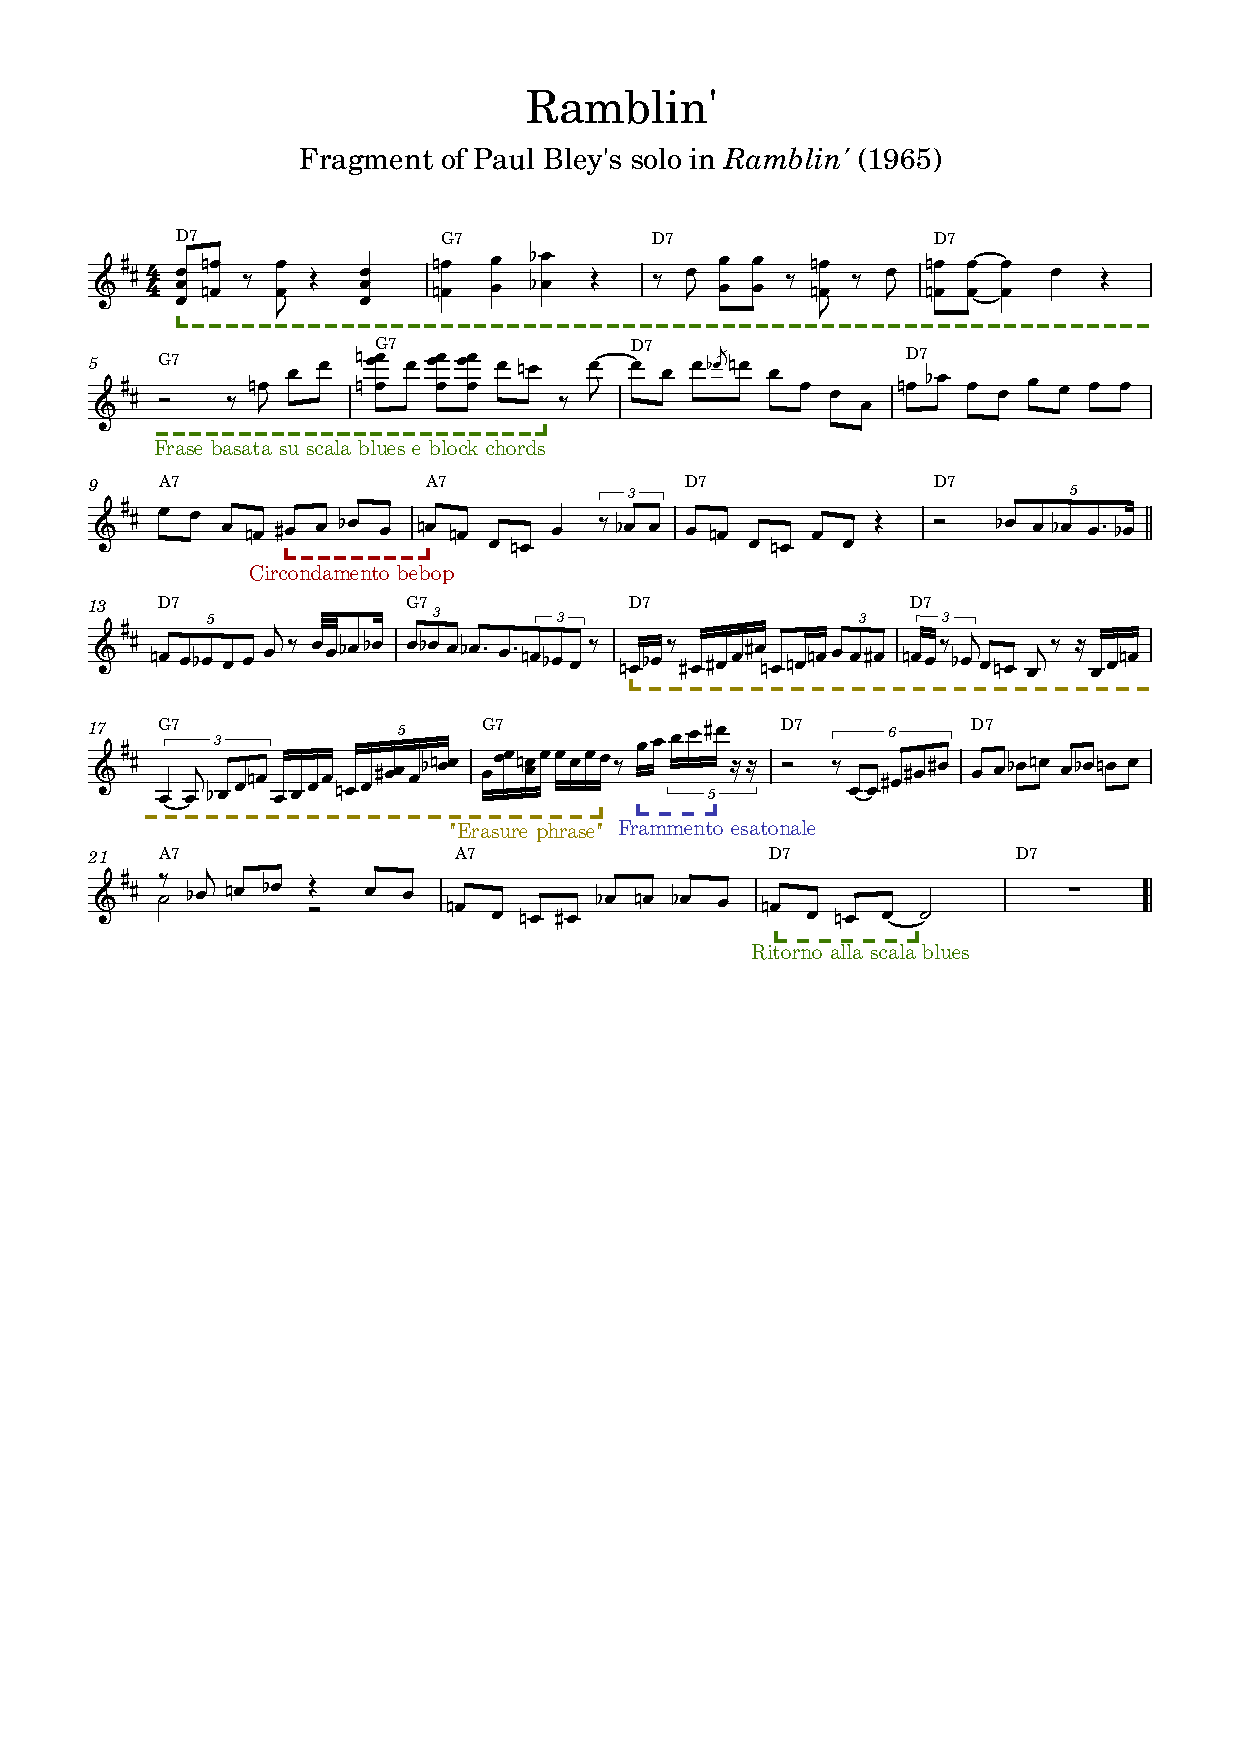
\includegraphics[clip,trim=1cm 13cm 1cm 3.5cm, width=\textwidth]{ramblin analysis.pdf}
	\caption{Ultimi due chorus di solo di pianoforte in \textit{Ramblin'}.}
	\label{fig:ramblin}
\end{figure}
Il blues è uno dei capisaldi dell'estetica di Coleman, per il quale costituiva sia un punto di partenza personale (come ex sassofonista di Rhythm \& Blues) sia culturale, nell'ambito di una musica che guarda a un ritorno alle radici dell'espressione afroamericana\footcite[38]{Cogswell1989}. Non stupisce quindi che anche Bley (seppur chiaramente per motivi diversi) torni così spesso e con tale limpidità al linguaggio blues. Dopotutto lui stesso riflette, a fronte della domanda di Arrigo Cappelletti sul suo rapporto con la tradizione blues:
\begin{fquote}
	Beh, il blues è un ottimo punto di partenza per poter suonare tutte le forme di jazz. Quindi quando suoni frasi orientate al blues sei abbastanza certo che finirai sul tracciato del jazz.\footcite[135]{cappelletti}
\end{fquote}
\section{In silenzio con Jimmy}
Oltre a Coleman, l'altra figura che Bley piazza nel suo pantheon di ispirazioni è Jimmy Giuffre\footcite{hamilton}. Il fatto che il pianista ponga queste due figure, ambedue pionieri e artefici di lavori all'apparenza così radicalmente diversi, è significativo dei punti in comune tra i due artisti.\par
L'interesse di Giuffre per la musica da camera\footcite[389]{johnston} lo 

\addcontentsline{toc}{chapter}{Appendice: materiale trascritto}
\addcontentsline{toc}{section}{All the things you are}
\appendix
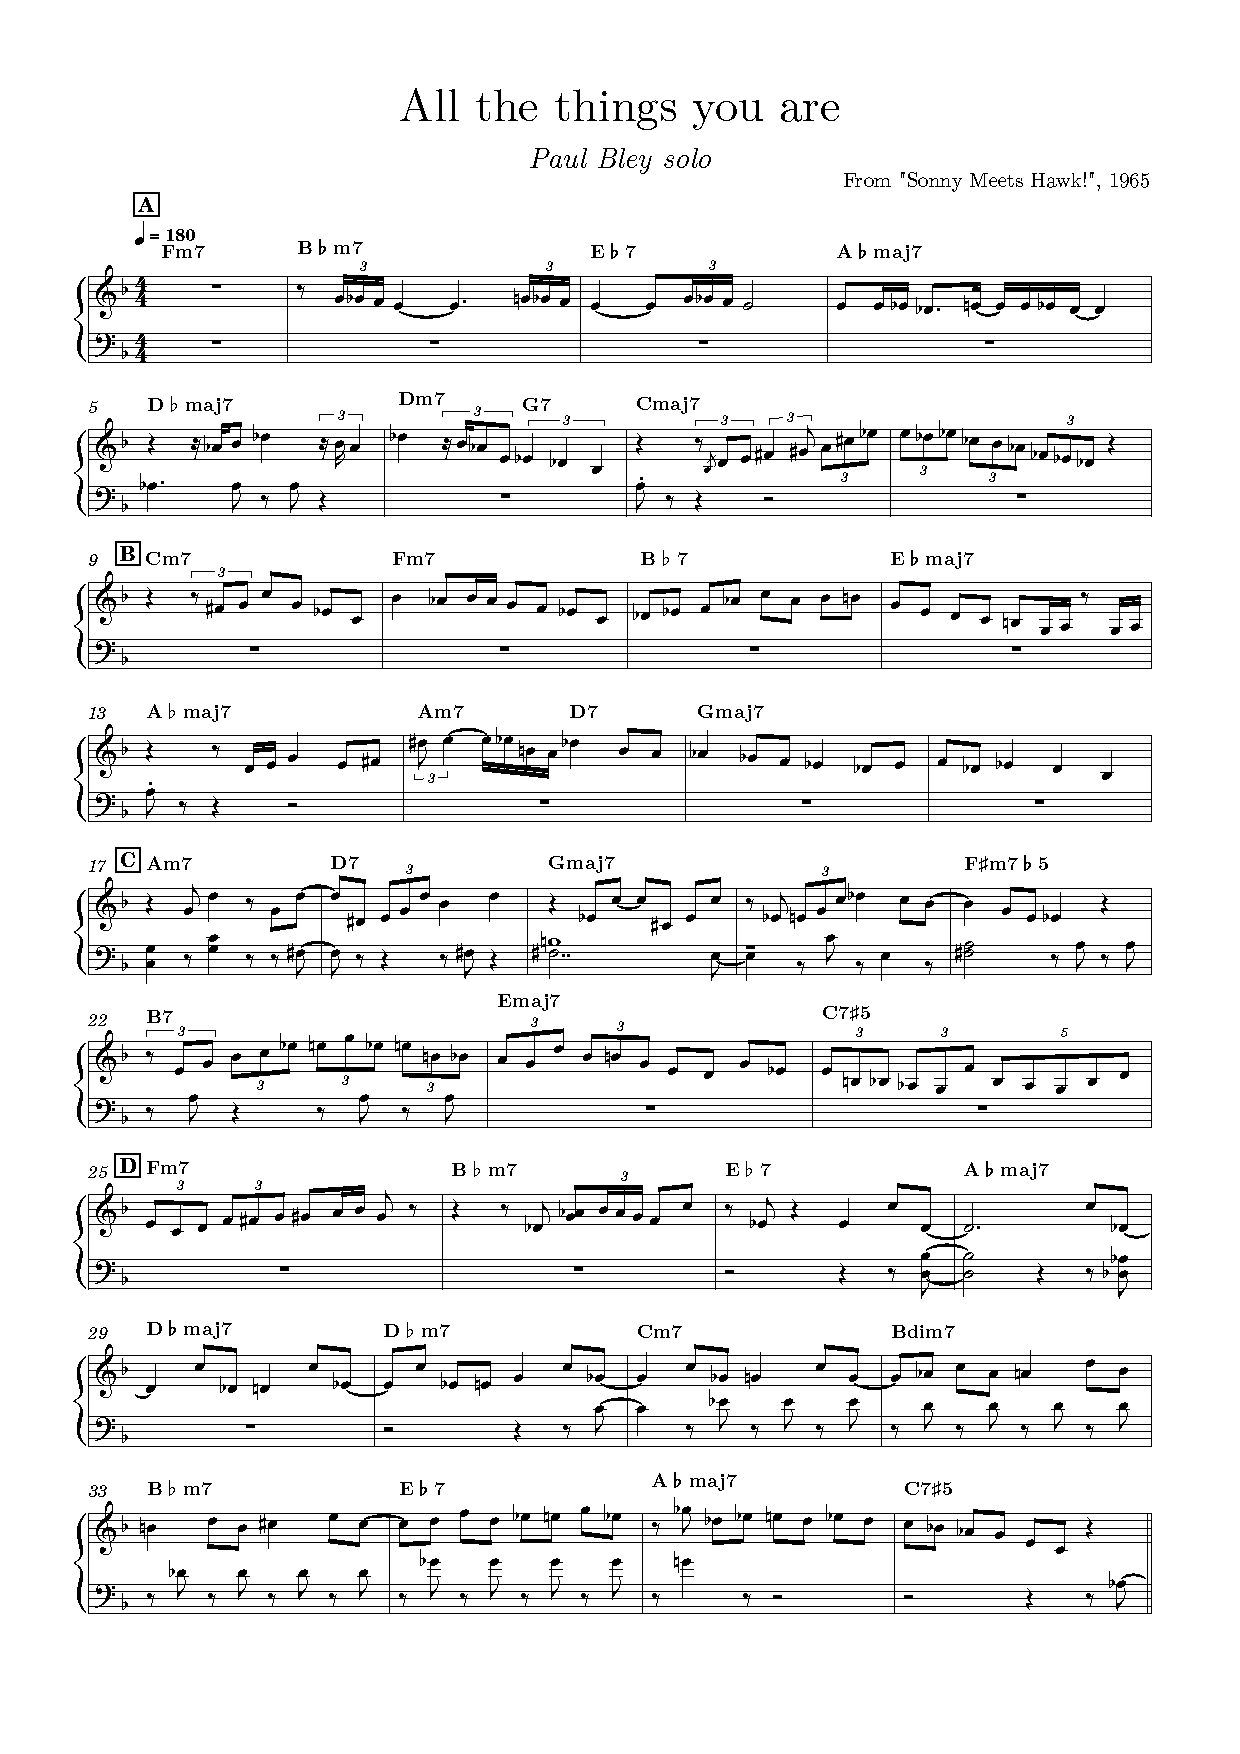
\includepdf[pages=-,pagecommand={},scale=0.9]{things_vanilla}
